%% bare_jrnl.tex
%% V1.4b
%% 2015/08/26
%% by Michael Shell
%% see http://www.michaelshell.org/
%% for current contact information.
%%
%% This is a skeleton file demonstrating the use of IEEEtran.cls
%% (requires IEEEtran.cls version 1.8b or later) with an IEEE
%% journal paper.
%%。
%% Support sites:
%% http://www.michaelshell.org/tex/ieeetran/
%% http://www.ctan.org/pkg/ieeetran
%% and
%% http://www.ieee.org/


%%*************************************************************************
%% Legal Notice:
%% This code is offered as-is without any warranty either expressed or
%% implied; without even the implied warranty of MERCHANTABILITY or

%% FITNESS FOR A PARTICULAR PURPOSE! 
%% User assumes all risk.
%% In no event shall the IEEE or any contributor to this code be liable for
%% any damages or losses, including, but not limited to, incidental,
%% consequential, or any other damages, resulting from the use or misuse
%% of any information contained here.
%%
%% All comments are the opinions of their respective authors and are not
%% necessarily endorsed by the IEEE.
%%
%% This work is distributed under the LaTeX Project Public License (LPPL)
%% ( http://www.latex-project.org/ ) version 1.3, and may be freely used,
%% distributed and modified. A copy of the LPPL, version 1.3, is included
%% in the base LaTeX documentation of all distributions of LaTeX released
%% 2003/12/01 or later.
%% Retain all contribution notices and credits.
%% ** Modified files should be clearly indicated as such, including  **
%% ** renaming them and changing author support contact information. **
%%*************************************************************************


% *** Authors should verify (and, if needed, correct) their LaTeX system  ***
% *** with the testflow diagnostic prior to trusting their LaTeX platform ***
% *** with production work. The IEEE's font choices and paper sizes can   ***
% *** trigger bugs that do not appear when using other class files.       ***                          ***
% The testflow support page is at:
% http://www.michaelshell.org/tex/testflow/

%
\documentclass[conference]{pvsctran}
%
% If IEEEtran.cls has not been installed into the LaTeX system files,
% manually specify the path to it like:
% \documentclass[journal]{../sty/IEEEtran}

%\input epsf
\usepackage{graphicx}
%\usepackage[dvipdfmx]{graphicx} % for michiko
\usepackage{hyperref} 
%\usepackage{graphicx}
\usepackage{amssymb}
\usepackage{amsmath}
\usepackage[super]{nth}
\usepackage{multicol}
% Add by Zhao
\usepackage{cite}
\usepackage{amsthm,amsfonts}
\usepackage{xcolor,color}
% \usepackage{caption2}
%\usepackage{graphicx}
\usepackage{enumerate}
\usepackage{multirow}
\usepackage{subcaption}
\usepackage[utf8]{inputenc}
\usepackage[ruled]{algorithm2e}
\usepackage[colorinlistoftodos]{todonotes}
\newtheorem{definition}{Definition}
\def\BibTeX{{\rm B\kern-.05em{\sc i\kern-.025em b}\kern-.08em
    T\kern-.1667em\lower.7ex\hbox{E}\kern-.125emX}}
% correct bad hyphenation here
\hyphenation{op-tical net-works semi-conduc-tor}

%In final version, please replace the following two definitions
\newcommand{\michiko}{\textcolor{black}}
%\newcommand{\michiko}{\textcolor{black}}
\newcommand{\zhao}{\textcolor{black}}

\captionsetup[subfigure]{justification=justified,singlelinecheck=false}
\captionsetup[figure]{justification=justified,singlelinecheck=false}


\begin{document}

\title{ A Rapid Feasibility Checking for Reconfiguration of Mismatched PV Arrays}

\author{ \IEEEauthorblockN{\large Dafang Zhao, Fukuhito Ooshita, and Michiko Inoue}
\IEEEauthorblockA{\large Nara Institute of Science and Technology, Japan \\ Email:\{zhao.dafang.yu7, f-oosita, kounoe\}@is.naist.jp}}

\setlength{\columnsep}{0.25in}


% make the title area
\maketitle


\begin{abstract}
%\boldmath
  Power generation efficiency of photovoltaic (PV) arrays is significantly affected by partial shading and PV cell damage.
  Partial shading or PV cell damage induces mismatched power generation among PV panels and causes an efficiency loss of power generation.
  Power losses of mismatched PV arrays can be recovered by reconfiguring connection of PV panels.
  In this paper, we introduce a \textit{feasibility check problem} of PV panel configuration.
  This problem identifies whether a connection among PV panels can be configured from a given PV module level solution.
  We also propose an algorithm for the \textit{feasibility check problem}.
  The experimental results demonstrate that the proposed algorithm can identify feasible configurations more than 32,000X faster than the exhaustive search with around 0.6\% errors. 
\end{abstract}

\begin{IEEEkeywords}
photovoltaic, feasibility, reconfiguration, mismatch
\end{IEEEkeywords}

\IEEEpeerreviewmaketitle



\section{Introduction}\label{Sec1}
As fossil fuel depletion and environmental pollution become more serious, green and renewable energy has become necessary for a sustainable society and environment. 
Photovoltaic (PV) systems receive significant attention since the sun has unlimited energy and PV arrays can be easily scaled up. 
However, due to the nature of PV cell, which is a basic component of a PV array, PV arrays are sensitive to partial shading and PV cell damage. 
PV cells could not uniformly generate power when they experience different irradiances or some of them have physical defects, and such a mismatched condition might accelerate heating and aging of PV cells and cause further damaging.
To prevent PV cells from damaging, bypass diodes are usually placed in PV arrays and they are turned on in mismatched conditions.
However, the operation of bypass diode will cause a number of PV cells to stop deliver power,
\michiko{and it will hence result in a significant loss of power generation.}

% it will introduce voltage drop which cause PV panel mismatched.
% However, it causes a significant loss of power generation. 

PV arrays are hierarchically constructed such that a group of PV cells form a PV module, a group of PV modules form a PV panel, and a group of PV panels form a PV array. 
Power generation of mismatched PV arrays can be recovered by reconfiguring connection of these components. 
Fig.\ref{compare} shows an example of power generations of a PV array with a partial shading. 
We distributed shading cells non-uniformly to a PV array with 3 $\times$  4 PV panels and applied power simulation. 
Before reconfiguration, \michiko{there are} multiple \michiko{peaks in a power - voltage curve with similar power levels,} while, after we reconfigured connection among PV panels, 
\michiko{some peaks exhibit much higher power levels than others and the }%
%MPPs has reduced and 
% power generation increased by 35\%.
% power generation increased by 35\%.
\zhao{maximum output power increased by 35\%}.

Though several reconfiguration methods have been proposed, most works consider reconfiguration in PV cell or PV module level \cite{nguyen2008adaptive,wang2014architecture,storey2013improved,storey2014optimized,udenze2018reconfiguration}. 
However, cell level reconfiguration requires a significantly high computation time and a large number of switches for reconfiguration. 
In addition, they require a special PV panels with capability of switching, and cannot be applied to the system constructed with standard PV panels. 
From a practical view, reconfiguration of connection among PV panels is a realistic solution since a PV panel is manufactured as a physical one panel with two terminals and PV panels can be flexibly interconnected. 
\begin{figure}[t]
\centering
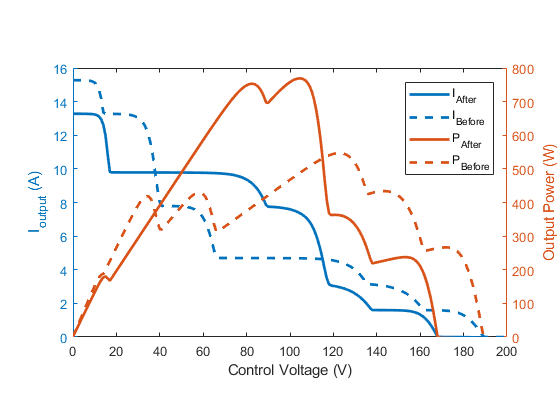
\includegraphics[width=9cm]{../fig/compare.png}
% \captionstyle{flushleft}
\caption{Power generation before and after reconfiguration}
\label{compare}
\end{figure}

Reconfiguration in PV panel level has been investigated~\cite{carotenuto2015evolutionary,hu2017non,orozco2016optimized}. 
A PV array reconfiguration using genetic algorithm (GA) was proposed in~\cite{carotenuto2015evolutionary}. Though it can give a new configuration, computing cost is significantly high and the algorithm cannot generate the best configuration precisely.  
Hu et al. also addressed PV panel reconfiguration where they formulate a nonlinear integer programming problem to optimize power generation by reconfiguration~\cite{hu2017non}.
Orozco-Gutierrez et al. proposed an efficient and effective reconfiguration method~\cite{orozco2016optimized} where it first selects candidates of configurations using the product of approximated currents and voltages,
then finds the best one with precise power simulation. 
However, these candidates are specified in a PV module level though PV modules could not be fully reconfigured. Actually, we found that some of configuration candidates are not able to be realized. However, the paper~\cite{orozco2016optimized}  does not show any systematic way to identify such a feasibility. 

In this paper, we propose an algorithm to rapidly check feasibility that a given configuration candidate is actually able to form by given PV panels. 
The proposed method can efficiently check the feasibility while identifying most feasible cases accurately. 
The experimental results demonstrate the effectiveness of the proposed method \michiko{where} it can identify the feasibility of configurations \michiko{with a very small}   false negative \michiko{rate of} less than 1\%.


\section{Photovoltaic Array}\label{Sec2}

A PV system or PV array is composed of PV panels that have two terminals of plus and minus and can be interconnected.
There are two common connection styles for PV arrays, \textit{series-parallel} array and \textit{total-cross-tied} array. 
In a series-parallel array, PV panels are connected in series, and multiple series connections are connected in parallel. 
In a total-cross-tied array, parallel connections of PV panels are connected in series. 
In this paper, we focus on series-parallel arrays, however the basic idea of the proposed method can be applied also to total-cross-tied arrays. 
Hereafter, we simply call a series-parallel array a \textit{PV array}. 

Figure \ref{model} shows an example of a PV array. 
A PV array is a parallel connection of (PV) strings where a string is a series connection of PV panels. 
A PV panel is a series connection of PV modules, and a PV module is a parallel connection of a series of PV cells and a bypass diode. 
A typical commercial PV panel is composed of three PV modules each of which has 12-24 PV cells. 
A PV module can generate power for a given voltage according to its I-V characteristics as shown in Fig.\ref{fig:IV}(a - c). 
The I-V characteristics is affected by irradiance level and physical damage of PV cells. 
\michiko{Figure \ref{fig:IV}(a - c) also show} a typical degradation of a I-V characteristics where generated \michiko{currents are reduced} with some ratio while keeping the voltage range. 
When a PV panel has a partial shade, that is its PV modules have different irradiance levels and hence different I-V characteristics, the PV panels might have multiple peaks (maximum power points, MPPs) in power generation as shown in Fig.\ref{fig:IV}(d). 

To find out accurate I-V characteristics of a PV panel, we need to apply a time consuming power simulation. 
However, we can roughly understand I-V characteristics of a PV panel (and also a string) as follows. 
When a control voltage is low, PV modules with high irradiance level are active while PV modules with low irradiance level are inactive with turning on their bypass diodes.
In this case, a high current can flow in the PV panel. When control voltage is increasing, some of bypass diodes become turning off and the corresponding PV modules become active. 
In that case, the current flow in the panel is determined by current of module with lowest irradiance level, and generated power sometimes increases and sometimes decreases.
% the current level is reduced and generated power sometimes increases and sometimes decreases. 
The generated power at MPPs can be roughly estimated. 
In Fig.\ref{fig:IV}(d), one PV panel has three PV modules with different irradiance levels. 
\michiko{Current levels at MPPs} for these modules are 4.3A, 3.0A, and 1.5A, respectively. 
\michiko{Voltage levels} at MPPs are roughly 20V, 44V, \michiko{and} 66V in Fig.\ref{fig:IV}(d), those are roughly multiples of a voltage of MPP for one PV module (around 20V in this case). 
At the first MPP (MPP1), only one PV module with \michiko{a current of 4.3A} is active at a control voltage of 22V, so the generated power is 94.6W. 
At the second MPP (MPP2), two PV modules with currents of 4.3A and 3.0A are active at a control voltage of 44V. 
In this case, the current level of the PV panel is 3.0A since two PV panels are connected in series and they have to have the same current level, and the generated power is 132W.
At the third MPP (MPP3), the current level of the PV panel is 1.5A at a control voltage of 66V, and the generated power is 99W. 

In a PV array, we have two constraints. 
PV panels in the same string have the same current level, while all the strings have the same control voltage. 
When considering reconfiguration of PV panel connection, we should find out the best configuration while considering these constraints. 

\begin{figure}[]
    \centering
    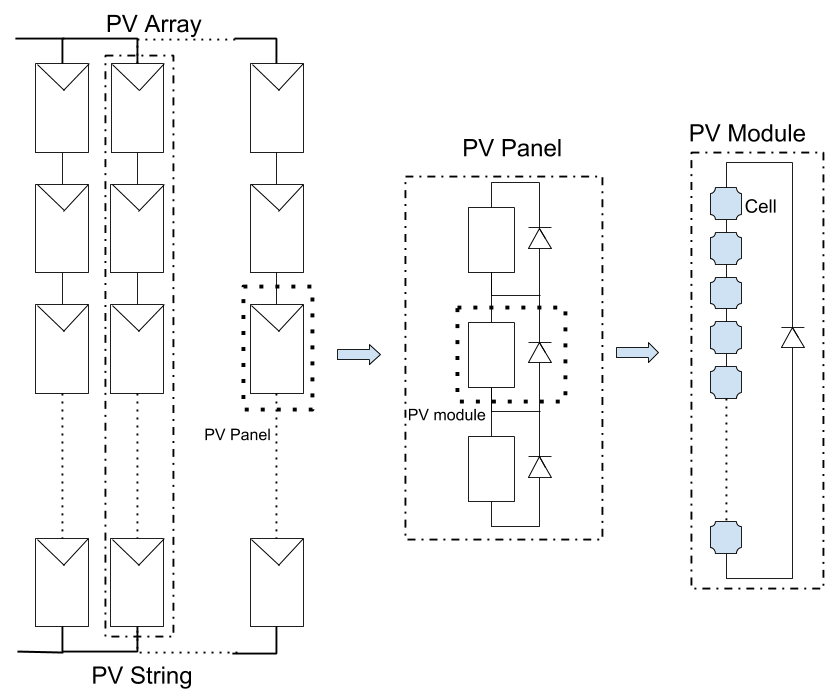
\includegraphics[width=9cm]{../fig/module.png}
    \caption{PV array, string, module and panel}
    \label{model}
\end{figure}

\begin{figure}
     \centering
    \begin{subfigure}[b]{2.7cm}
        \centering
        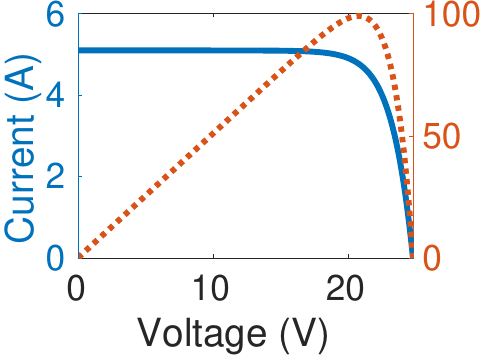
\includegraphics[width=\linewidth]{../fig/m_1.png}
        \caption{PV module 1}
     \end{subfigure}
     \begin{subfigure}[b]{2.7cm}
        \centering
        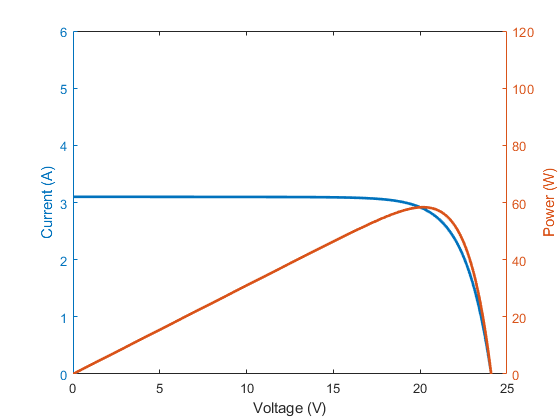
\includegraphics[width=\linewidth]{../fig/m_2.png}
        \caption{PV module 2}
     \end{subfigure}
     \begin{subfigure}[b]{2.7cm}
        \centering
        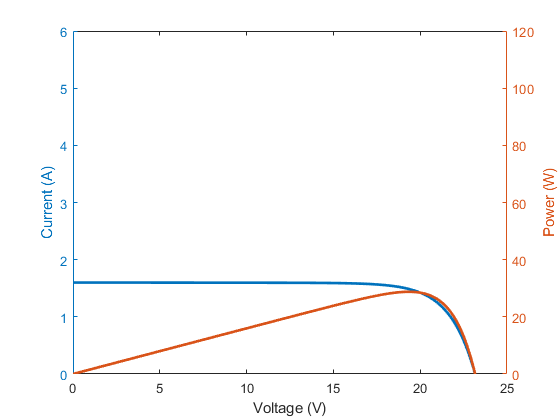
\includegraphics[width=\linewidth]{../fig/m_3.png}
        \caption{PV module 3}
    \end{subfigure}
    \hfill
    \begin{subfigure}[b]{9cm}
        \centering
        \vspace{3mm}
        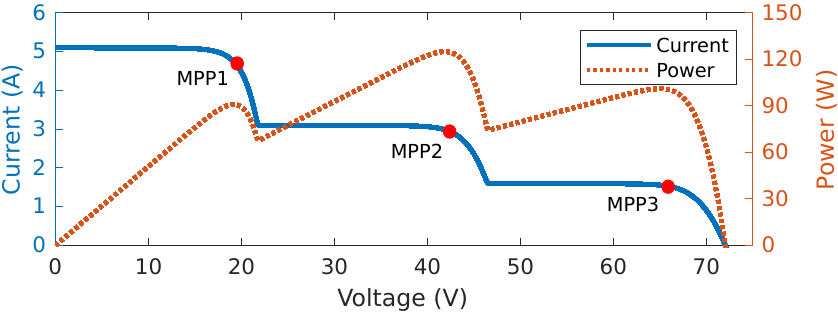
\includegraphics[width=9cm]{../fig/panel.png}
        \caption{PV panel}
    \end{subfigure}
    \caption{I-V characteristics}
    \label{fig:IV}
\end{figure}






\section{Orozco-Guierrez's method}\label{Sec3}
In this section, we briefly introduce a method proposed by Orozco-Guierrez et al.\cite{orozco2016optimized} as the most related work to this paper.
Orozco-Guierrez et al. proposed an efficient reconfiguration algorithm for mismatched PV arrays. 
The method utilizes information of MPPs of every PV panel that is extracted using an online monitoring \cite{carotenuto2014online} and a power estimation \cite{orozco2015fast}.

\begin{table}[t]
% \caption{Extracted currents of MPPs}
% \caption{EXTRACTED CURRENTS OF MPPS}
% \label{tab:monitored}
\centering
\caption{}
\centerline{EXTRACTED CURRENTS OF MPPS}
\vskip5pt
\begin{tabular}{c|rrrr}
\hline\hline
       &    	\multicolumn{4}{c}{Panels}								\\
	&	\multicolumn{1}{c}{$P1$}	&	\multicolumn{1}{c}{$P2$}	&	\multicolumn{1}{c}{$P3$}	&	\multicolumn{1}{c}{$P4$}	\\ \hline
MPP1	&	3.10A	&	3.09A	&	0.52A	&	2.47A	\\ \hline
MPP2	&	2.98A	&	2.55A	&	0.50A	&	1.53A	\\ \hline
MPP3	&	1.55A	&	2.48A	&	0.46A	&	0.48A	\\ \hline
\end{tabular}
\label{tab:monitored}
\end{table}

\begin{table}[t]
% \caption{Approximated currents of MPPs}
% \caption{APPROXIMATED CURRENTS OF MPPS}
% \label{tab:approximated}
\centering
\caption{}
\centerline{APPROXIMATED CURRENTS OF MPPS}
\vskip5pt
\begin{tabular}{c|rrrr}	
\hline\hline
       &    	\multicolumn{4}{c}{Panels}	\\
	&	\multicolumn{1}{c}{$P1$}	&	\multicolumn{1}{c}{$P2$}	&	\multicolumn{1}{c}{$P3$}	&	\multicolumn{1}{c}{$P4$}	\\ \hline
MPP1	&	3A	&	3A	&	0.5A	&	2.5A	\\ \hline
MPP2	&	3A	&	2.5A	&	0.5A	&	1.5A	\\ \hline
MPP3	&	1.5A	&	2.5A	&	0.5A	&	0.5A	\\ \hline
\end{tabular}
\label{tab:approximated}
\end{table}

\begin{table}[t]
% \caption{Maximum number of active modules}
% \caption{MAXIMUM NUMBER OF ACTIVE MODULES}
% \label{tab:modules}
\centering
\caption{}
\centerline{MAXIMUM NUMBER OF ACTIVE MODULES}
\vskip5pt
\begin{tabular}{c|rrrr|r}	
\hline\hline
       &    	\multicolumn{4}{c|}{Panels}	& \\									
	&	\multicolumn{1}{c}{$P1$}	&	\multicolumn{1}{c}{$P2$}	&	\multicolumn{1}{c}{$P3$}	&	\multicolumn{1}{c}{$P4$} &	\multicolumn{1}{|c}{total}	\\ \hline
3A	&	2	&	1	&	0	&	0 & 3	\\ \hline
2.5A	&	2	&	3	&	0	&	1 & 6	\\ \hline
1.5A	&	3	&	3	&	0	&	2 & 8	\\ \hline
0.5A	&	3	&	3	&	3	&	3 & 12	\\ \hline
\end{tabular}
\label{tab:modules}
\end{table}


For the method in \cite{orozco2016optimized}, first, close values \michiko{of extracted currents or voltages are} approximated and grouped into a small number of classes so that the number of possible combinations, or a search space, is reduced.
Then possible combinations of reconfiguration are enumerated.
For each candidate configuration \michiko{its generated} power value \michiko{is} estimated by \cite{orozco2015fast} along with careful estimation of possible errors.
For example, Table \ref{tab:monitored} shows extracted currents for 4 panels each of which has 3 modules, and they are approximated into four current levels as shown in Table \ref{tab:approximated}. 
% Then currents and voltages of MPPs are approximated and grouped into a small number of classes so that the number of possible combinations, or a search space, is reduced.
As mentioned in Section \ref{Sec2}, if some panel has $m$ MPPs with current level of $I$ or larger, $m$ modules can be active with current level of $I$. 
Table \ref{tab:modules} shows the maximum number of active modules for each current level.
Control voltage for one PV model is approximated to 20V.
Approximated power values for possible configurations are shown in Table \ref{tab:powers}. 
% Then power values are approximated for possible configurations. 
Table \ref{tab:powers} shows an example to form a PV array with two strings,
%where power value is simply multiplied PV array current with control voltage .
\michiko{where control voltages are approximated as multiples of 20V (the number of active modules per string times 20V), and power values of strings are obtained as products of current and voltage values. For example, when current levels of two strings are 3A and 2.5A and the number of active modules per string \zhao{are} 3, the control voltage is 60V, and two strings generate powers of $3\mbox{A} \times 60\mbox{V} = 180\mbox{W}$ and $2.5\mbox{A} \times 60\mbox{A} = 150\mbox{W}$, and the total generated power is \zhao{approximated about} 330W.}

\michiko{When constructing an approximated power matrix like Table~\ref{tab:powers}, the possibility that an array can be formed for a given current sequence and the number of active modules per string (it is called \textit{feasibility}) is examined.}
The method \michiko{provides} a simple feasibility check as follows. 

\textbf{(Feasibility 1)}\footnote{In~\cite{orozco2016optimized}, only the case of $n=2$ is considered, and we extended the condition to general $n$. }%
For the $n$-th highest current level $I_{n}$ \michiko{in a current sequence for strings}, the number of active modules in a configuration candidate is $N(I_{n}) / n$ or less,
where $N(I)$ is the total number of active modules for a current level $I$. 

For example, consider a candidate current pair (3A, 2.5A). In this case, the highest and the second highest current levels are 3A and 2.5A, respectively, and the total number of active modules for 3A and 2.5A are 3 and 6, respectively (see Table \ref{tab:modules}). Therefore, the number of active modules in the first string is 3 or less, and the number of active modules in the second string is also $ 6/2  = 3$ or less. Consequently, the number of active modules per string is at most 3 for a candidate current pair (3A. 2.5A). Table \ref{tab:powers} has values in the cells when Feasibility 1 is satisfied. 

The method finds the largest power value from possible candidate configurations (330W for current pair (3A, 2.5A) with three active modules in this case) and evaluates the case more precisely along with the cases with close values to the best value since the analysis are given with approximated values. In the case of Table \ref{tab:powers}, 330W, 320W and 300W are selected for further evaluation. 


\begin{table*}[t]
% \caption{Approximated power}
  \caption{}
  \centerline{APPROXIMATED POWER}
  \vskip5pt
\label{tab:powers}
\centering
\begin{tabular}{c|rrrrrrrrrrr}
\hline\hline	
\# modules & 	\multicolumn{10}{c}{currents sequence for strings (A)} \\ 																
per string		&	\multicolumn{1}{c}{(3,3)}	&	\multicolumn{1}{c}{(3,2.5)}	&	\multicolumn{1}{c}{(3,1.5)}	&	\multicolumn{1}{c}{(3,0.5)}	&	\multicolumn{1}{c}{(2.5,2.5)}	&	\multicolumn{1}{c}{(2.5,1.5)}	&	\multicolumn{1}{c}{(2.5,0.5)}	&	\multicolumn{1}{c}{(1.5,1.5)}	&	\multicolumn{1}{c}{(1.5,0.5)}	&	\multicolumn{1}{c}{(0.5,0.5)}	\\ \hline
	1	&	120W	&	110W	&	90W	&	70W	&	100W	&	80W	&	60W	&	60W	&	40W	&	20W	\\ \hline
	2	&	-	&	220W	&	180W	&	140W	&	200W	&	160W	&	120W	&	120W	&	80W	&	40W	\\ \hline	3	&	-	&\textbf{330W}&	270W	&	210W	&	\textbf{300W}	&	240W	&	180W	&	180W	&	120W	&	60W	\\ \hline
4	&	-	&	-	&	-	&	-	&	-	&	\textbf{320W}	&	240W	&	240W	&	160W	&	80W	\\ \hline
	 5	&	-	&	-	&	-	&	-	&	-	&	-	&	\textbf{300W}	&	-	&	200W	&	100W	\\ \hline
	6	&	-	&	-	&	-	&	-	&	-	&	-	&	-	&	-	&	240W	&	120W	\\ \hline
\end{tabular}
\end{table*}

\section{Feasibility}
In the method\cite{orozco2016optimized}, to execute a power simulation for a PV array, we need to assign panels into strings to realize a candidate configuration. 
For example, a candidate configuration for a current pair (2.5A, 2.5A) with 3 active modules is realized by assign panel P2  to the first string and panels P1 and P4 to the second string as shown in Fig.\ref{fig:feasible-configuration}. 
However, we could not find \michiko{any} feasible assignment for a current pair (3A, 2.5A) with 3 active modules or a current pair (2.5A, 1.5A) with 4 active modules though they are expected to generate higher powers 330W or 320W. 
That is, the condition Feasibility 1 is necessary but not sufficient to give a actual feasibility result.

\begin{figure}[b]
    \centering
    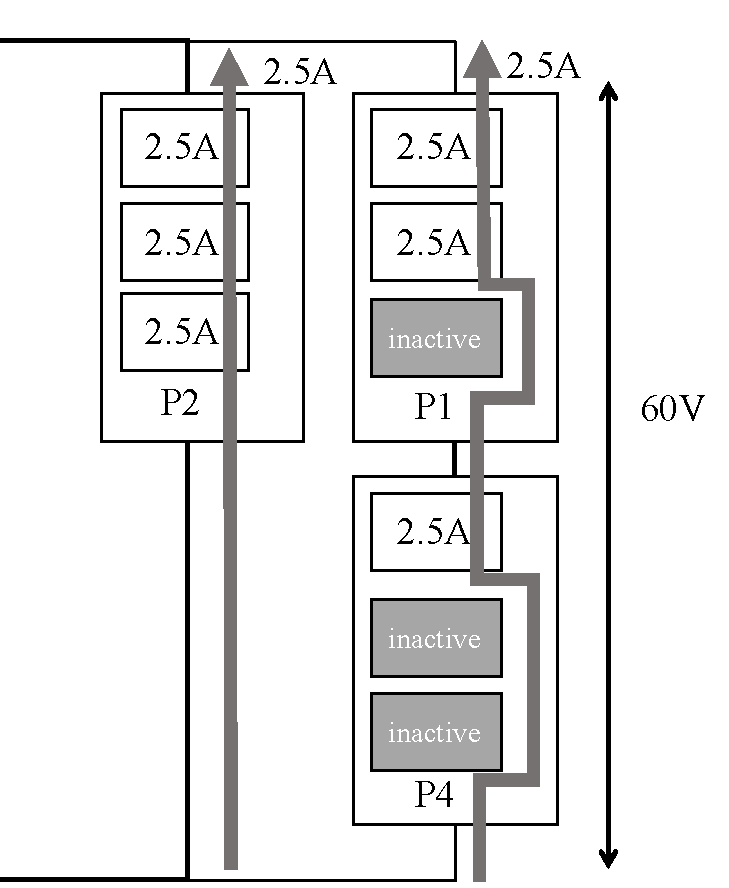
\includegraphics[width=0.6\linewidth]{../fig/feasible-configuration-vertical.pdf}
    \caption{Feasible configuration for a current pair (2.5A, 2.5A) with 3 active modules.}
    \label{fig:feasible-configuration}
\end{figure}

Now we will define the feasibility. For a PV array $A$ with $s$ strings, let $M_{A,i}(I)$ denote the number of modules that can be active with a current level $I$ in the $i$-th string.
Let $Q = (Q_{1},Q_{2},\ldots ,Q_{s})$ be a sequence of currents required for strings. 
A sequence of currents $Q$ is feasible with $m$ modules if and only if it is possible to form a PV array $A$ such that 
\begin{equation}
M_{A,i}(Q_{i}) \geq m
\end{equation}
holds for each string $i (1 \leq i \leq s)$.

\section{An algorithm to identify feasibility}\label{Sec5}
\subsection{Feasibility Problem}\label{Sec5_1}
In this section, we propose an algorithm to identify feasibility.
First we will formulate the feasibility problem that identifies the feasibility for a given current sequence and the number of active modules per string as follows.

\textit{Definition 1} (\textit{Feasibility Problem}):\\
\textbf{Input}: Information of MPPs (approximated values), a current sequence $Q$, the number of $m$ of active modules per-string.\\
%\newline
\textbf{Output}: Whether $Q$ with $m$ modules is feasible or not.

\subsection{Outline of the algorithm}
In the proposed algorithm, we try to configure a PV array and identify the feasibility of configuration.
For a given current sequence $Q = (Q_{1},Q_{2},\ldots ,Q_{s}) (Q_{i} \geq Q_{j} \mbox{\ if\ } i \leq j)$, we will assign panels to strings in the order of $Q_{1},Q_{2},\ldots ,Q_{s}$. 
When selecting a panel to a string, we will consider how much we lose an opportunity that the panel is more effectively used for other current level. 
For example, if we select Panel $P1$ in Table \ref{tab:modules} for a string with a current level 3A, two modules can be active while the remaining one module becomes inactive. 
The remaining one module still is not active if $P1$ is used for a current level 2.5A, while it can be active if it is used for current level 1.5A or 0.5A. 
We will consider that, when selecting $P1$ for a current level 3A, we do not have any loss for a current level 2.5A but lose one module for 1.5A and 0.5A. 
The algorithm select panels so as to minimize such losses. 

Let $M_{p}(I)$ denote the number of modules that can be active at current level $I$ in a PV panel $p$. 
For a given current sequence $Q = (Q_{1},Q_{2},\ldots ,Q_{s}) (Q_{i} \geq Q_{j} \mbox{\ if\ } i \leq j)$, 
a loss of selecting a panel $p$ at the $k-1$-th string for the $k$-th string is defined as 
$Loss(p,k) = M_{p}(Q_{k}) - M_{p}(Q_{k-1})$. 

To assign panels for the $n$-th string, the following steps are applied. Let $m$ be the required number of active modules.
\begin{enumerate}
\item Sort unselected PV panels in a lexicographically ascending order of $Loss(p,n+1)$, $Loss(p,n+2)$,$\ldots$, $Loss(p,s)$ and $M_{p}(Q_{n})$.
\item Select PV panels until selecting $m$ or more active modules for a current level $Q_{n}$.
\item Cancel redundant PV panels so that the number of active modules at a current level $Q_{n}$ is minimized.
\item Swap selected PV panels with unselected PV panels so that the number of selected PV panels is minimized.
\end{enumerate}

Before explaining more details, we first show an example.
Table \ref{tab:proposed-example} shows how to select PV panels for the first string where the required number $m$ of active modules is 5. 
Panels are sorted by $Loss$ and $M_{p}(Q_{1})$ (the number of active modules for the first string) in the order of $P1$, $P2$, $\ldots$, $P7$. 
In the example, panels $P2$ to $P6$ are at the same loss level $(1,0)$. 
PV panels are selected for each loss level. First, $P1$ is selected, then panels at the second loss level are selected in the order of $P2$, $P3$, $\ldots$. After selecting until $P5$, the number of active modules exceed $m (=5)$. In this case, if some redundant panels exist, these panels are canceled. In the example, $P4$ is canceled. Finally, if some of selected PV panels can be swapped with less number of unselected panels, they are swapped. In the example, $P2$ and $P3$ are swapped with $P6$. Consequently, three panels $P1$, $P5$ and $P6$ are selected. 

\begin{table}[t]
% \caption{An example of the proposed method ($m = 5$)}
  \caption{}
  \centerline{AN EXAMPLE OF THE PROPOSED METHOD ($ m = 5$)}
  \vskip5pt
\begin{center}
\begin{tabular}{c|c|ccccc|c}\hline \hline
                               & \multicolumn{7}{c}{Panels}  \\
                               &  \multicolumn{1}{c}{$P1$}    & $P2$   & $P3$    & $P4$    & $P5$   & \multicolumn{1}{c}{$P6$}            & $P7$             \\ \hline
$M_{p}(Q_1)$        & 1     & 1     & 1     & 1     & 2    & 2    & 1              \\ \hline
$M_{p}(Q_2)$        & 1     & 2     & 2     & 2     & 3    & 3    & 2              \\ \hline
$M_{p}(Q_3)$        & 1     & 2     & 2     & 2     & 3    & 3    & 3              \\ \hline
$Loss(p,2)$           & 0     & 1     & 1     & 1     & 1    & 1    & 1    \\ \hline
$Loss(p,3)$           & 0     & 0     & 0     & 0     & 0    & 0    & 1    \\ \hline\hline
step 2        & $\surd$ & $\surd$ &$\surd$ &$\surd$ &$\surd$ & & \\ \hline
step 3      & $\surd$ & $\surd$ &$\surd$ & &$\surd$ & & \\ \hline
step 4       & $\surd$ &  & & &$\surd$ & $\surd$ & \\ \hline         
\end{tabular}
\end{center}
\label{tab:proposed-example}
\end{table}

\subsection{Algorithm}
\michiko{The proposed algorithm first obtains loss levels for each panel, and assigns panels for strings in the order of $1,2,\ldots ,s$ where $Q_{i} \geq Q_{j} (i \leq j)$ holds for a required current sequence $Q = (Q_{1},Q_{2},\ldots ,Q_{s})$. The pseudo code is given in Algorithm~\ref{alg1}.
To assign panels to the $n$-th highest current $Q_{n}$, the following 4 steps are applied.}

Step 1 sorts unselected panels in a lexicographically ascending order of $Loss(p,n+1)$, $Loss(p,n+2)$,$\ldots$, $Loss(p,s)$ and $M_{p}(Q_{n})$.
This sorting step \michiko{gives} a basic \michiko{selection} priority for all unselected panels. 
\michiko{A panel with less losses for higher current levels are preferred. For example, a panel $P1$ has $(Loss(P1,2), Loss(P1,3)) = (0,0)$, that is there is no loss for further assignment, and it has the highest priority. The last value $M_{p}(Q_{n})$ (the number of active modules at a current level $Q_{n}$ in panel $p$) is used to select the minimum number of modules for a required current level, and it will be described in Step 3.}
%A panel with uniformly irradiance distribution is preferred over non-uniformly irradiance distributed panel.

Step 2 selects sorted panels one by one until reaching the required number of active modules.
In this selection step, panel with no active modules are skipped.
% That will cut the computational space in the step 3 and step 4.
% Step 1 sorts unselected panels (with modules that can be active for the target current), and Step 2 selects panels one by one in the sorted order until reaching the required number of active modules.  

Step 3 optimizes the number of active modules. 
In Step 3, if the number of active modules exceeds the required number $m$, redundant panels \zhao{are} canceled if exist. 
A panel is \textit{redundant} if the number of active modules is still $m$ or more even if \zhao{the} panel is canceled.
Redundant panels are searched \michiko{for each loss level}. 
Starting with a loss level where the last panel is selected, we check the number of active modules $M_{p}(Q_{n})$ for each panel $p$ 
where $Q_{n}$ is a required current level for the current string.
Redundant panels are selected and canceled from panels with less number of $M_{p}(Q_{n})$ in the same loss level. 
If \michiko{the number of active modules} still exceeds $m$ after canceling,
the same procedure is applied to the previous loss level.
% we will go to the previous loss level and try to cancel panels.
This procedure is repeated until selecting an exactly $m$ active modules or checking all the loss levels.
\michiko{This step accurately finds redundant panels if exist in the following reason. Since the number of active modules in one panel is 0, 1, 2, or 3 \zhao{as assumed in Section \ref{Sec2}} and panels are selected from panels with less active modules in the same loss level, if the number of active modules exceed $m$, the surplus is 1 or 2. That means, the last selected panel has 2 or 3 active modules, and panels with 1 or 2 active modules have already selected if exist.}

Step 4 optimizes the number of selected panels.
In Step 4, we swap selected panels and an unselected panel in the same loss level to reduce the number of selected panels.
There are 3 swap rules as shown in Table \ref{tab:swap}.
This swap procedure \michiko{keeps the number of active modules while reducing the number of panels. The step increases the number of unselected panels and hence increase the flexibility for succeeding selection.}
%will minimum the total module losses and further more reduce the number of panels.
% Pseudo codes are given below to give details to summarize the process of proposed algorithm.
%\textbf{\textit{Algorithm 1}} shows a pseudo code of the proposed algorithm.

\begin{table}[ht]
% \caption{Swap rule}
  \caption{}
  \centerline{SWAP RULE}
  \vskip5pt
\label{tab:swap}
\centering
\begin{tabular}{c|c}
\hline\hline
\multicolumn{2}{c}{The numbers of active modules} \\
selected panels & unselected panels \\ \hline
1, 1, 1 & 3 \\ \hline
1, 1 & 2 \\ \hline
1, 2 & 3 \\ \hline
\end{tabular}
\end{table}

\begin{algorithm}[htp]
\caption{Feasibility Check Problem}
\label{alg1}
\LinesNumbered
\SetKwInOut{Input}{Input}  
\Input{\\
  \textit{$Q = Q_1, Q_2, \ldots , Q_s$}: required current for each string; \\
  \textit{$m$}: the minimum number of active modules per string;\\
  \textit{$M_{p}$}: the number of active modules in each panel \textit{p};\\
  %\textit{P}: Number of panels; 
  \textit{s}: the number of strings;}
\SetKwInOut{Output}{Output}
\Output{Feasibility Result;%\\
        %Conf: Configuration Result;
        }
\For{\textup{each string} $ k (2 \leq k \leq s)$ \textup{and panel} $p$}{$Loss(p,k) = M_{p}(Q_{k}) - M_{p}(Q_{k-1})$}
\For{j = 1 to s}
    {{\If{$\sum M_{p}(Q_{j})$ \textup{for unselected panels} $< m$}
       {\textup{\textbf{return :}} Feasibility = NO}}
     $PS$ = a set of unselected panels with $M_{p}(Q_{j}) > 0$;\\
     // step 1\\
     sort $PS$ in a lexicographically ascending order of $Loss(p,j+1)$, $Loss(p,j+2)$, $\ldots$, $Loss(p,s)$, $M_{p}(Q_{j})$;\\
     // step 2\\
     select panels in the order in $PS$ until $\sum M_{p}(Q_{j})$ for selected panels $\geq m$;\\
     //step 3\\
     group selected panels $LV_{1}$, $LV_{2}$,$\ldots$, $LV_{h}$ with loss level ($LV_{1}$ is the lowest level);\\
     \For{i = h to 1}
     {find and cancel redundant panels in $LV_{i}$ in the order in $PS$}
     //step 4\\
     \For{i = h to 1}
     {apply swap rules for selected panels in $LV_{i}$ and an unselected panel in the same loss level}
    }
    \textup{\textbf{return :}} Feasibility = YES
\end{algorithm}

\section{Evaluation}\label{Sec6}
%Although the pilot example refers to three strings only, the extension of the method to any number of parallel connected string is the same.

\michiko{To evaluate the proposed method, we prepared MPP informations of 100 mismatched PV arrays and applied our algorithm. We also applied an exhaustive searching algorithm for comparison.
MPP information is setup as follows for each PV array. 
Each PV array has 6 - 24  panels and the number of PV panels is randomly determined. 
Three current values are randomly assigned to the three modules in each panel from 3 - 8 current values, where the number of possible current values are also randomly determined for each PV array.
% \zhao{\large \textbf{Is that means: Current value for PV modules in each PV panel are randomly assigned from 3 - 8 current values.}}
The number of strings after reconfiguration is 3 - 6 and it is randomly determined for each PV array.}

\michiko{We first applied the method~\cite{orozco2016optimized} to select configuration candidates. Condition \textbf{Feasibility 1} is applied to exclude a part of infeasible configurations, and then configurations that generate more than 77\% of the maximum power are selected from the remainings as candidates as mentioned in~\cite{orozco2016optimized}.  In our experiments, 486 candidates are selected from 100 PV arrays as shown in Table~\ref{result_compare}. That is, for each PV arrays, 4 - 5 candidates are selected in average.}

\michiko{Table~\ref{result_compare} shows the results of feasibility checking by the proposed algorithm and the exhaustive search.} 
%To evaluate the performance of  proposed algorithm, 
%we compare the result with exhaustive searching algorithm for 100 random shadow distributed PV arrays. For each PV array, 6 - 24 PV panels are connected into 3 - 6 PV strings. For each PV panel, it will has 3 - 8 working current values.
%The computational time required for finding optimal configuration and accuracy of feasibility judgment in the proposed algorithm and exhaustive search algorithm are compared in Table \ref{result_compare}. 
%As shown in Table \ref{result_compare},
% proposed algorithm achieved less computing time compare with exhaustive search algorithm and with high accuracy.  
%from 100 PV arrays, 486 configuration candidates are selected where each candidate is specified with a required current sequence for strings and the number of active modules per string.
Since the exhaustive search checks all the combinations of panel connections for each configuration candidate, it accurately identifies the feasibility of every configuration. % but that takes a lot of time.
\michiko{Though the exhaustive search identified total 327 feasible configurations, the proposed method identified 324 configurations and 3 configurations are misidentified. 
The proposed algorithm had a few false negative cases, but its rate was less than 1\%.
That is, it can correctly identify feasibility for most cases. 
Indeed, the proposed algorithm found at least one candidate configuration as feasible among 4 - 5 candidates for each PV arrays. }

The calculation was performed using an Intel i7-4770 Quad-Core processor and 16 GB of RAM memory.
The time used by the proposed feasibility check method was 3ms, which is significantly lower than the 98s needed by the exhaustive search algorithm.
%On the other hand, the proposed method misidentifying only 3 feasible negative cases, the error rate is less than 1 \%.
% On the other hand, the proposed algorithm misidentifying only 3 feasible negative cases with rapidly (more than 32,000X faster) feasibility checks speed.

In conclusion, the proposed method provides a solution for checking the feasibility of PV configurations with an error lower than 1\% but execution time are significantly lower than the one required by exhaustive search algorithm.
% Each PV array has 4 or 5 candidates and our algorithm indeed found PV panel connection for each PV array.

\begin{table}[htbp]
\caption{}
\begin{center}
\begin{tabular}{ccc}
\multicolumn{3}{c}{\begin{tabular}[c]{@{}c@{}}COMPARISON BETWEEN EXISTED METHODS\\ AND PROPOSED ALGORITHM\end{tabular}}                                         \\ \hline \hline
\multicolumn{1}{c|}{}                         & \multicolumn{1}{c|}{Proposed Algorithm} & \begin{tabular}[c]{@{}c@{}}Exhaustive search \\ Algorithm\end{tabular} \\ \hline
\multicolumn{1}{c|}{Number of PV Array}       & \multicolumn{2}{c}{100}                                                                                         \\ \hline
\multicolumn{1}{c|}{Number of MPP candidates} & \multicolumn{2}{c}{486}                                                                                       \\ \hline
\multicolumn{1}{c|}{Feasible Candidates}      & \multicolumn{1}{c|}{324}              & 327                                                                   \\ \hline
\multicolumn{1}{c|}{Infeasible Candidates}    & \multicolumn{1}{c|}{162}              & 159                                                                   \\ \hline
\multicolumn{1}{c|}{Error Rate}               & \multicolumn{1}{c|}{0.62\%}            & 0\%                                                                    \\ \hline
\multicolumn{1}{c|}{Ave. times per Array}     & \multicolumn{1}{c|}{0.003s}            & 98s                                                                 
\end{tabular}
\label{result_compare}
\end{center}
\end{table}

% \begin{table}[ht]
% \caption{PV Cell Parameters}
% \begin{center}
% \begin{tabular}{c|c}
% \hline \hline
% Parameter             & Value  \\ \hline
% Short-Circuit Current & 0.66A  \\
% MPP-Current           & 0.58A  \\
% Open-Circuit Voltage  & 280V   \\
% MPP-Voltage           & 215V  \\
% Max Power Output      & 124.7W 
% \end{tabular}
% \end{center}
% \label{PV_cell_par}
% \end{table}

\section{Conclusion}

Power generation of mismatched PV arrays can be recovered by reconfiguring connection of PV panels.
In this paper, we introduced a feasibility check problem to configure PV panel connections from PV module connections and proposed an algorithm that efficiently and effectively solves the problem. 
The experimental results show that the proposed algorithm can identify feasible configurations more than 32,000X faster than the exhaustive search with around 0.6\% errors. 
The proposed method is useful to identify or configure actual PV panel connections from PV module level specifications or connections. 
Since there are many works of PV module level reconfiguration and PV panel level reconfiguration using PV module level optimization as an intermediate solution, the proposed algorithm is useful to actually find PV panel connections from PV module level solutions.
PV panel level reconfiguration is a practical and realistic solution for PV arrays composed of standard PV panels, 
and the proposed method contributes to find efficient and effective solution for PV panel level reconfiguration.
% Following these instructions will improve the quality of your paper and the PVSC Proceedings. If you have comments, please contact \url{Publications@ieee-pvsc.org}. Please direct questions regarding the electronic submission process to \url{help@SPLTrak.com}. 

% conference papers do not normally have an appendix

% use section* for acknowledgment



% conference papers do not normally have an appendix


% use section* for acknowledgement



% trigger a \newpage just before the given reference
% number - used to balance the columns on the last page
% adjust value as needed - may need to be readjusted if
% the document is modified later
%\IEEEtriggeratref{8}
% The "triggered" command can be changed if desired:
%\IEEEtriggercmd{\enlargethispage{-5in}}

% references section
\renewcommand\refname{Reference}
\bibliographystyle{ieeetr}
\bibliography{reference}
% can use a bibliography generated by BibTeX as a .bbl file
% BibTeX documentation can be easily obtained at:
% http://www.ctan.org/tex-archive/biblio/bibtex/contrib/doc/
% The IEEEtran BibTeX style support page is at:
% http://www.michaelshell.org/tex/ieeetran/bibtex/
%\bibliographystyle{IEEEtran}
% argument is your BibTeX string definitions and bibliography database(s)
%\bibliography{IEEEabrv,../bib/paper}
%
% <OR> manually copy in the resultant .bbl file
% set second argument of \begin to the number of references
% (used to reserve space for the reference number labels box)
% \begin{thebibliography}{1}
% \small

% \bibitem {Yamaguchi}
% M. Yamaguchi, A. Khan, S.J. Taylor, M. Imaizumi, T. Hisamatsu, and S. Matsuda, ``A detailed model to improve the radiation-resistance of Si space solar cells,\emph{Fundamentals of Solar Cells} vol. 46, pp. 2133-2138, 1999.

% \bibitem {Hovel}
% H. J. Hovel and J. M. Woodall, ``The effect of depletion region recombination currents on the efficiencies of Si and GaAs solar cells'', \emph {in 10th IEEE Photovoltaic Specialist Conference}, p. 25, 1973.

% \bibitem {Fahrenbruch}
% A. L. Fahrenbruch and R. H. Bube, \emph{Fundamentals of Solar Cells}, New York: Academic Press, 1983.

% %\bibitem{IEEEhowto:kopka}
% %H.~Kopka and P.~W. Daly, \emph{A Guide to \LaTeX}, 3rd~ed.\hskip 1em plus
% %  0.5em minus 0.4em\relax Harlow, England: Addison-Wesley, 1999.

% \end{thebibliography}
%\smallskip
%Note: For the Summary paper submission only, references to the authors own work must be redacted to preserve the new double-blind reviewing requirements.





% that's all folks
\end{document}


